%==================================================================
%==================================================================
\subsection*{Binary block-models}
%==================================================================
\frame{ \frametitle{Stochastic block-model (SBM, 1/2)}
  
  \paragraph{Undirected network:} Cluster structure
  $$
  \includegraphics[width=.6\textwidth]{\figeco/mangwet-SBM-fit.pdf}
  $$
}

%==================================================================
\frame{ \frametitle{Stochastic block-model (SBM, 2/2)}
  
  \paragraph{Nested structure:} do clusters actually exist?
  $$
  \includegraphics[width=.6\textwidth]{\figeco/stmarks-SBM-fit.pdf}
  $$
}

%==================================================================
\frame{ \frametitle{Latent block-model (LBM)}

  \paragraph{Asymmetric version of SBM:} $n$ top nodes (pollinators), $m$ bottom nodes (plants)
  $$
  Y_{ij} = \Ibb\{ i \rightarrow j\}
  $$

  \bigskip \pause
  \paragraph{Model:}
  \begin{itemize}
   \item $K$ top groups, $L$ bottom groups
   \item $Z^1_i = k $ if top node $i$ belongs to group $k$
   \item $Z^2_j = \ell$ if bottom node $j$ belongs to group $\ell$
   \item Connection probability
   $$
   P(Y_{ij} = 1 \mid Z^1_i = k, Z^2_j = \ell) = \gamma_{k\ell}
   $$
  \end{itemize}

}

%==================================================================
\frame{ \frametitle{LBM for plants-pollinators}

  \paragraph{Bipartite network:} UK plant-pollinator network
    
    
  \hspace{-0.05\textwidth}
  \begin{tabular}{p{.35\textwidth}p{.45\textwidth}}
    \begin{tabular}{p{.4\textwidth}}
      \begin{itemize}
        \item $n = 485$ pollinators \\
        $m = 499$ plants \\ ~
        \item $\widehat{K} = 19$ pollinator groups \\
        $\widehat{L} = 15$ plant groups \\ ~ 
        \item $\gamma_{k\ell} =$ prob. interaction btw \\
        a pollinator from group $k$ and \\
        a plant from group $\ell$
      \end{itemize}
    \end{tabular}
    &
    \begin{tabular}{p{.45\textwidth}}
      \includegraphics[width=.6\textwidth]{\figeco/plant_pollinator_interactions_for_potential_networks_2018-LBM-fit.pdf}
    \end{tabular} 
  \end{tabular}
    
}

%==================================================================
%==================================================================
\subsection*{Extensions}
%==================================================================
\frame{ \frametitle{Valued network with covariates}
  
\begin{itemize}
 \item $n = 51$ tree species \refer{MRV10}, 
 \item $Y_{ij} =$ number of shared parasites, 
 \item $x_{ij} =$ (taxonomic, geographic, genetic distances)
\end{itemize}

\begin{tabular}{cc}
 \begin{tabular}{p{.5\textwidth}}
  \onslide+<2->{Without covariates: $\Pcal(e^{\gamma_{k\ell}})$  \\
  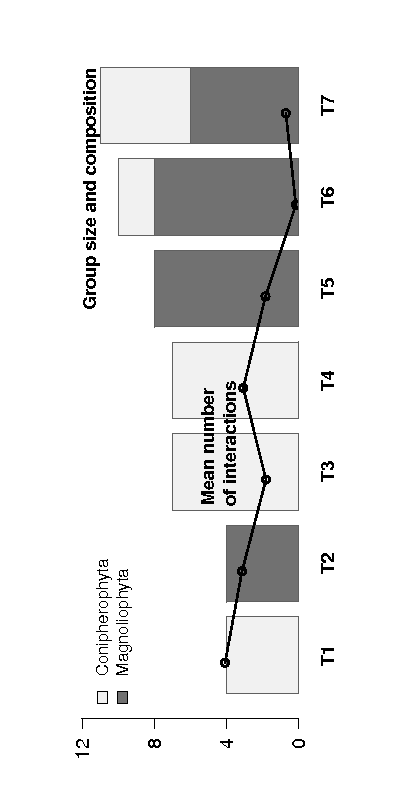
\includegraphics[height=.65\textheight, width=.35\textwidth, angle=270, trim=50 0 30 0, clip]{\fignet/MRV10_AoAS_Q7_group} \\
  ($\widehat{K} = 7$)
  }
  \end{tabular}
  & 
  \hspace{-.05\textwidth}
  \begin{tabular}{p{.5\textwidth}}
  \onslide+<3->{With covariates: $\Pcal(e^{\gamma_{k\ell} + \emphase{x_{ij}^\trans \beta}})$ \\
  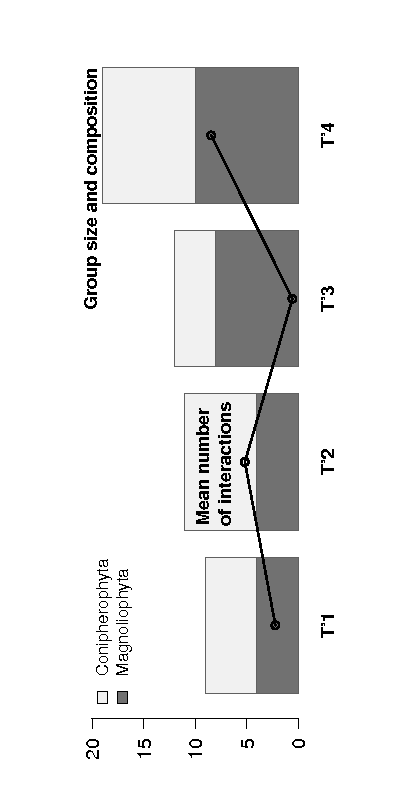
\includegraphics[height=.6\textheight, width=.35\textwidth, angle=270, trim=50 0 30 0, clip]{\fignet/MRV10_AoAS_Q4_group} \\
  ($\widehat{K} = 4$)
  }
 \end{tabular}
\end{tabular}

}

%==================================================================
\frame{ \frametitle{Dynamic SBM}

  \paragraph{Time-stamped network:} one network per day
  $$
  Y^t_{ij} = \text{ presence/absence of an interaction between $i$ and $j$ on day $t$}
  $$
  \ra Ex.: social contacts among onagers\refer{RSF15}
  
  \bigskip \bigskip \pause
  \paragraph{Dynamic version of SBM (dynSBM, \refer{MaM17}).} Group membership can vary along time
  $$
  Z_i^t = \text{ group of node $i$ on day $t$}
  $$
  
  \bigskip \pause
  \begin{tabular}{p{.4\textwidth}p{.5\textwidth}}
    \begin{tabular}{p{.4\textwidth}}
      \begin{itemize}
        \item $(Z_i^t)_t \sim$ Markov chain \\ ~
        \item $P(Y_{ij}^t = 1 \mid Z_i^t, Z_j^t) = \gamma_{Z_i^t, Z_j^t}$ \\ ~
        \item \url{dynsbm} R package
      \end{itemize}
    \end{tabular}
    &
    \begin{tabular}{p{.5\textwidth}}
      \includegraphics[width=.4\textwidth]{\fignet/MaM17-JRSSB-Fig8b}
    \end{tabular} 
  \end{tabular}
}

%==================================================================
\frame{ \frametitle{Multipartite network}

  \paragraph{Plant-animal interactions:} \refer{BBD19}
  \begin{itemize}
    \item $n = 141$ plants
    \item $m = 344$ animals ($m_1 = 173$ pollinators, $m_2 = 46$ frugivorous birds, $m_3 = 30$ ants)
    \item Interactions plants-others are recorded (presence / absence)
    \item Aim: define groups of plants having similar interaction profiles {\sl with the 3 sets of animals}
  \end{itemize}
  
  \bigskip \pause
  \begin{tabular}{p{.45\textwidth}p{.45\textwidth}}
    \begin{tabular}{p{.45\textwidth}}
      \paragraph{Multipartite SBM:} $K / (L_1, L_2, L_3)$ groups ~ \\ 
      \includegraphics[width=.45\textwidth]{\fignet/BBD19-ArXiv-Tab1} \\
      {\tiny $* =$ not plotted on the right panel}
    \end{tabular}
    &
    \begin{tabular}{p{.45\textwidth}}
      \includegraphics[width=.45\textwidth]{\fignet/BBD19-ArXiv-Fig2}
    \end{tabular} 
  \end{tabular}

}

% %==================================================================
% \frame{ \frametitle{And also..}
% 
%   \begin{itemize}
%    \item Multilayer: \refer{PPP17}
%    \item Spatial constraint: \refer{MPD14}
%   \end{itemize}
%   
% }
